\documentclass[compress, aspectratio=32]{beamer}
\usepackage[utf8]{inputenc}
\usepackage{graphicx} % Required for inserting images
\graphicspath{ {./images/} }
\usepackage{amsmath}
\usepackage{mathspec}
\usepackage{xeCJK}
\usepackage{multicol}
\usepackage{float}
\usepackage{soul}
\usepackage{hyperref}
\usepackage{caption}
\usepackage{subcaption}
\usepackage{ulem}
\usepackage{listings}
\usepackage[backend=biber, citestyle=authoryear, sorting=none]{biblatex}
\addbibresource{ref.bib}

\useinnertheme{circles}
\useoutertheme[subsection=true, footline=authortitle]{miniframes}
%\usecolortheme{seagull}
\usefonttheme{structurebold}

\setmainfont{Sabon LT Pro}
\setsansfont{SF Pro Display}
%\setmathfont(Digits,Latin){Goldman Sans}
\setmonofont{IBM Plex Mono}

\AtBeginSection[]
{
    
  \begin{frame}[allowframebreaks]
    
    \tableofcontents[currentsection]
    
  \end{frame}
}

% \AtBeginSubsection[]{
%     \begin{frame}[allowframebreaks]
%         \tableofcontents[currentsubsection]
%     \end{frame}
% }

\title[UI Dev]{Intro to Frontend Development}
\subtitle{with Flutter}
\author{Ben Cheng}
\institute{RISD ID}
\date{\today}

\setbeamertemplate{navigation symbols}{\insertframenumber/\inserttotalframenumber}
\setbeamertemplate{title page}{
    \vbox{}
    \vfill
    \begin{beamercolorbox}[sep=8pt,left]{title}
        \begin{columns}
            \begin{column}[]{0.7\textwidth}
                \usebeamerfont{title}\inserttitle\par
        \ifx\insertsubtitle\@empty
        \else
          \vskip0.25em
          {\usebeamerfont{subtitle}\usebeamercolor[fg]{subtitle}\insertsubtitle\par}%
        \fi   
            \end{column}
            \begin{column}[]{0.1\textwidth}
                
\includegraphics[width=\textwidth]{IDSB-logo.png}
            \end{column}
        \end{columns}
          
      \end{beamercolorbox}
    \vskip1em\par
    \begin{beamercolorbox}[sep=8pt,left]{author}
      \usebeamerfont{author}\insertauthor
    \end{beamercolorbox}
    \begin{beamercolorbox}[sep=8pt,left]{institute}
        \usebeamerfont{institute}\insertinstitute
    \end{beamercolorbox}
    \begin{beamercolorbox}[sep=8pt,right]{date}
        \usebeamerfont{date}\insertdate
    \end{beamercolorbox}\vskip0.5em
    {\usebeamercolor[fg]{titlegraphic}\inserttitlegraphic\par}
    \vfill
}

\definecolor{customColor}{RGB}{90, 158, 108}
\setbeamercolor*{palette primary}{fg=customColor!60!black,bg=white!85!customColor}
\setbeamercolor*{palette secondary}{fg=customColor!70!black,bg=white!60!customColor}
\setbeamercolor*{palette tertiary}{bg=customColor!80!black,fg=white!50!customColor}
\setbeamercolor*{palette quaternary}{fg=customColor,bg=white!20!customColor}

\setbeamercolor*{sidebar}{fg=customColor,bg=customColor!75!white}

\setbeamercolor*{palette sidebar primary}{fg=customColor!10!black}
\setbeamercolor*{palette sidebar secondary}{fg=white}
\setbeamercolor*{palette sidebar tertiary}{fg=customColor!50!black}
\setbeamercolor*{palette sidebar quaternary}{fg=white!10!customColor}

\setbeamercolor*{titlelike}{parent=palette primary}
\setbeamercolor{frametitle}{bg=white!90!customColor}
\setbeamercolor{frametitle right}{bg=white!60!customColor}

\setbeamercolor{block title}{parent=palette tertiary}
\setbeamercolor{block body}{bg=white!90!customColor}

\setbeamercolor*{item projected}{parent=palette primary}%fg=black,bg=black!20}

\setbeamercolor*{normal text}{fg=black,bg=white}
\setbeamercolor*{alerted text}{fg=black}
\setbeamercolor*{example text}{fg=black}
\setbeamercolor*{structure}{fg=black}

\setbeamercolor{author in head/foot}{parent=title in head/foot}

\lstdefinestyle{mystyle}{basicstyle=\ttfamily\scriptsize, numbers=left, frame=lines, breaklines=true, showstringspaces=false}
\lstset{style=mystyle}

\begin{document}

\frame{\titlepage}

\begin{frame}[allowframebreaks]{Outline}
    \tableofcontents
\end{frame}

\section{Layout and Design}
\begin{frame}
    \frametitle{Everything is a widget}
    and widgets are wrapped by widgets
    \begin{columns}
        \begin{column}{0.5\textwidth}
            \centering
            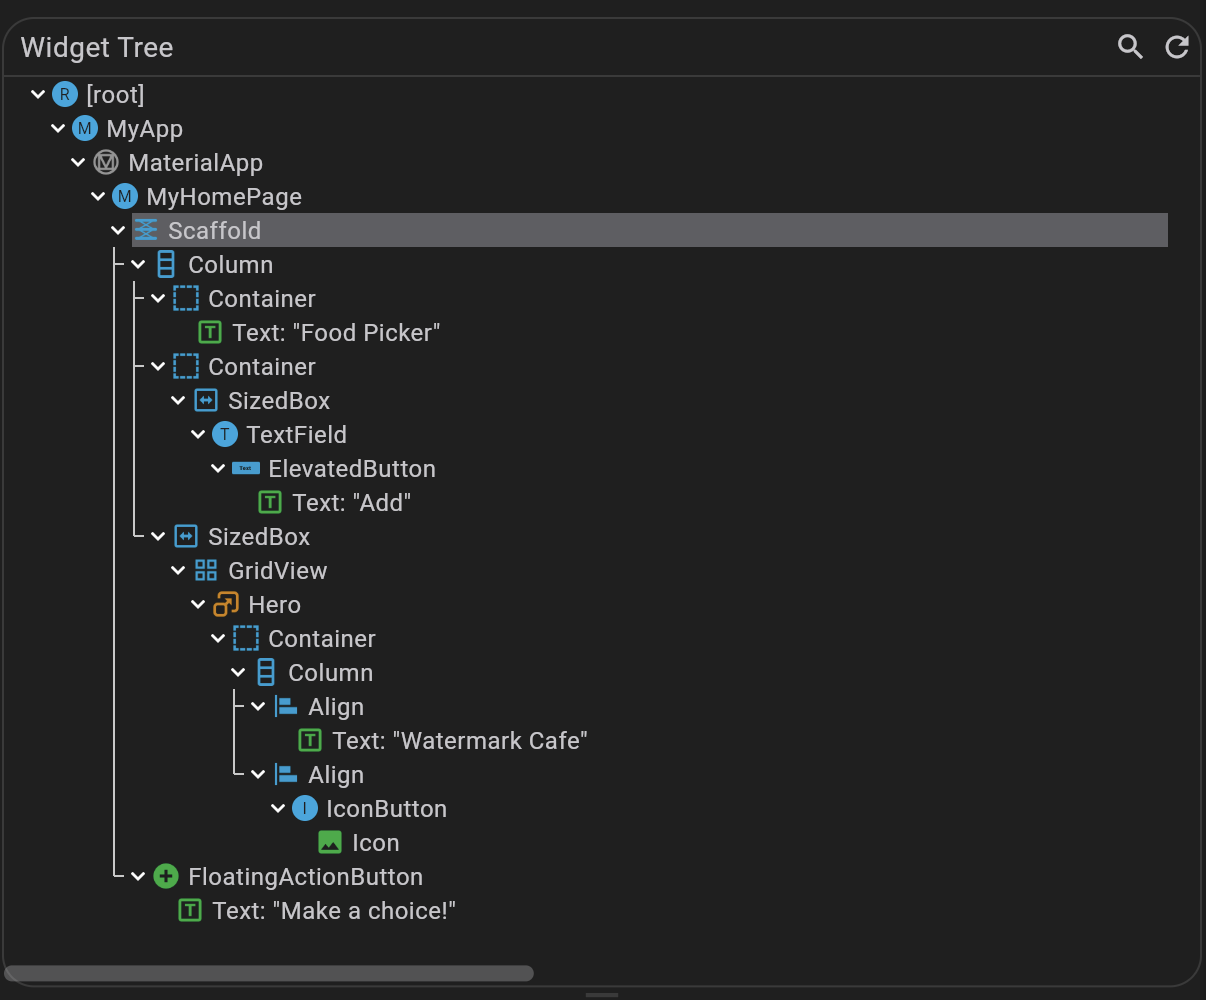
\includegraphics[width=0.8\textwidth]{widgettree.png}
        \end{column}
        \begin{column}[]{0.5\textwidth}
            \centering
            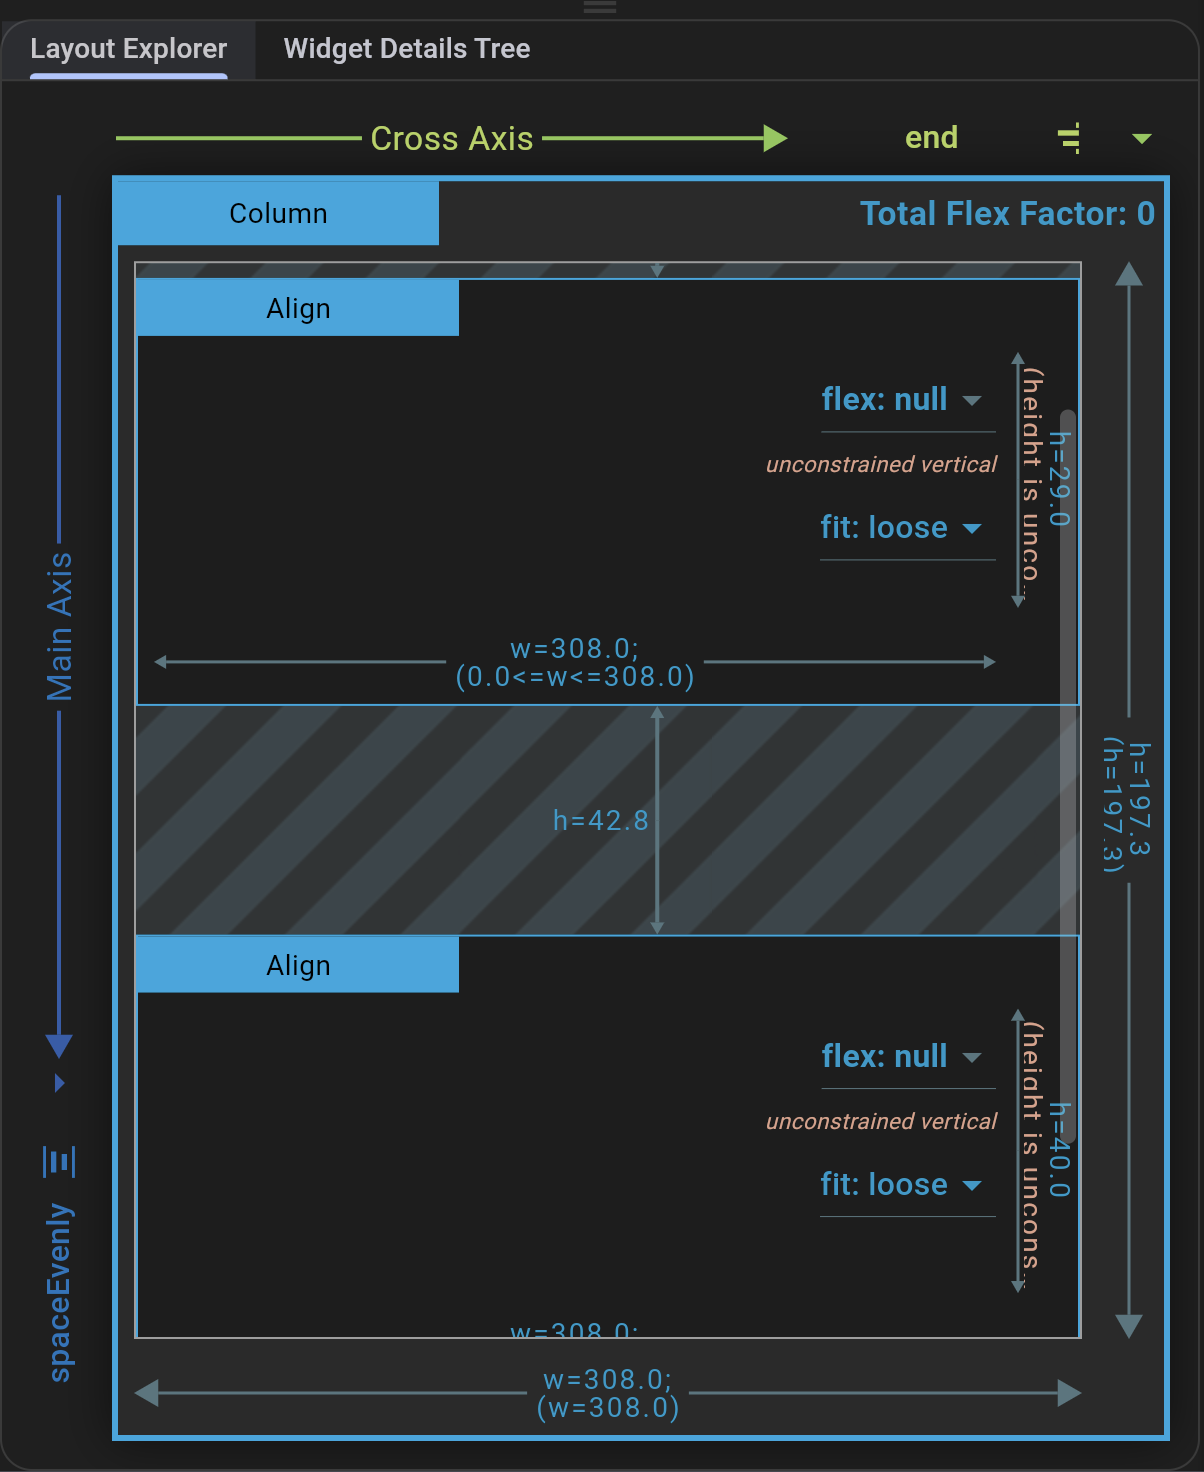
\includegraphics[height=0.7\textheight]{widget.png}
        \end{column}
    \end{columns}
\end{frame}

\begin{frame}
    \frametitle{Layout}
    \begin{columns}
        \begin{column}[]{0.4\textwidth}
           \begin{itemize}
        \item Column
        \item Row
        \item Flex
        \item Stack
    \end{itemize}
    \begin{itemize}
        \item Spacer
        \item Align
    \end{itemize} 
        \end{column}
        \begin{column}[]{0.6\textwidth}
            \centering
            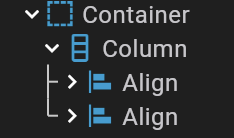
\includegraphics[width=0.8\textwidth]{column.png}
        \end{column}
    \end{columns}
    
\end{frame}
\begin{frame}[fragile]
    \frametitle{Container()}
    \begin{lstlisting}[language=c, firstnumber=140]
Container(
    padding: const EdgeInsets.all(12),
    decoration: BoxDecoration(
        borderRadius: const BorderRadius.all(Radius.circular(10)),
        color: Colors.deepPurple.shade100,
    ),
    \end{lstlisting}
    \begin{itemize}
        \item BoxDecoration: color, border, border radius, shadow, image, gradient, shape
        \item An alternative when you want to restrict size: SizedBox()
    \end{itemize}
\end{frame}

\begin{frame}[fragile]
    \frametitle{Google Fonts}
    \begin{lstlisting}[numbers=none]
flutter pub add google_fonts
    \end{lstlisting}
    \begin{lstlisting}[language=c, firstnumber=3]
import 'package:google_fonts/google_fonts.dart';
    \end{lstlisting}
    \begin{lstlisting}[language=c, firstnumber=100]
Text(
    "Food Picker",
    style: GoogleFonts.robotoSlab(
        textStyle: const TextStyle(
            fontWeight: FontWeight.w900, fontSize: 80, height: 1.1)),
    )
    \end{lstlisting}
\end{frame}

\section{Interaction}
\begin{frame}[fragile]
    \frametitle{Callback}
    \begin{lstlisting}[language=c, firstnumber=114]
ElevatedButton(
    child: const Text("Add"),
    onPressed: () => {
    _addOption( // a custom callback function declared earlier
        value: _optionTextEditingController.value.text)
    },
     ))
    \end{lstlisting}
\end{frame}
\begin{frame}[fragile]
    \frametitle{setState}
    Declaration of the custom call back function:
    \begin{lstlisting}[language=c, firstnumber=114]
void _addOption({required String value}) {
    setState(() {
        _options.add(value);
        _optionTextEditingController.clear();
    });
    }
    \end{lstlisting}        
\end{frame}

\begin{frame}[fragile]
    \frametitle{Update Where?}
    \begin{lstlisting}[language=c, firstnumber=151]
Text(
    _options[index], // actual text determined by the data in the list _options
    style: GoogleFonts.robotoSlab(
        textStyle: const TextStyle(fontSize: 20)),
    )
    \end{lstlisting}
\end{frame}

\section{Navigation}
\begin{frame}[fragile]
    \frametitle{Navigator}
    \begin{itemize}
        \item Routes (screens) are arranged as a stack.
        \item Push or pop to move between screens.
    \end{itemize}
    \begin{lstlisting}[language=c, firstnumber=80]
FloatingActionButton.extended(
    onPressed: () => {
        if (_options.isNotEmpty)
        {
            Navigator.push(context, MaterialPageRoute(builder: (context) {
            var choice = Random().nextInt(_options.length);
            return Result(result: _options[choice]);
            }))
        }
    },
    \end{lstlisting}
\end{frame}

\begin{frame}
\frametitle{Other Navigation Tools}
\begin{itemize}
    \item Page
    \item Routes
    \item Tabs
    \item (Deeplinks)
\end{itemize}
\end{frame}

\section{Animation}
\begin{frame}[fragile]
    \frametitle{GestureDetector()}
    Callbacks: onTapDown, onTapUp
    \begin{lstlisting}[language=c, firstnumber=201]
GestureDetector(
    behavior: HitTestBehavior.opaque,
    onTapDown: (details) {
    setState(() {
        scale = 1.075;
    });
    },
    onTapUp: (details) {
    setState(() {
        scale = 1;
    });
    },
    \end{lstlisting}
\end{frame}
\begin{frame}[fragile]
    \frametitle{Implicit Animation}
    \begin{enumerate}
        \item AnimatedContainer()
        \item Some properties of the widget are not constant
        \item Animation automatically triggered when properties change
    \end{enumerate}
    \begin{lstlisting}[language=c, firstnumber=219]
AnimatedContainer(
            duration: Durations.short2,
            height: scale * 400, // non-constant height
            width: MediaQuery.of(context).size.width * 0.75 * scale, // non-constant width
            child: Center(
                child: Text(
            widget.result,
            style: GoogleFonts.robotoSlab(
                textStyle: const TextStyle(fontSize: 40)),
            ))),
    \end{lstlisting}
\end{frame}
\begin{frame}
    \frametitle{Explicit Animation}
    When
    \begin{itemize}
        \item You want to ``manually'' trigger animation.
        \item You want the animation to run forever.
        \item You want different animation (duration, curve) for different property.
        \item Your animation has ``discontinuities''.
    \end{itemize}
\end{frame}

\end{document}